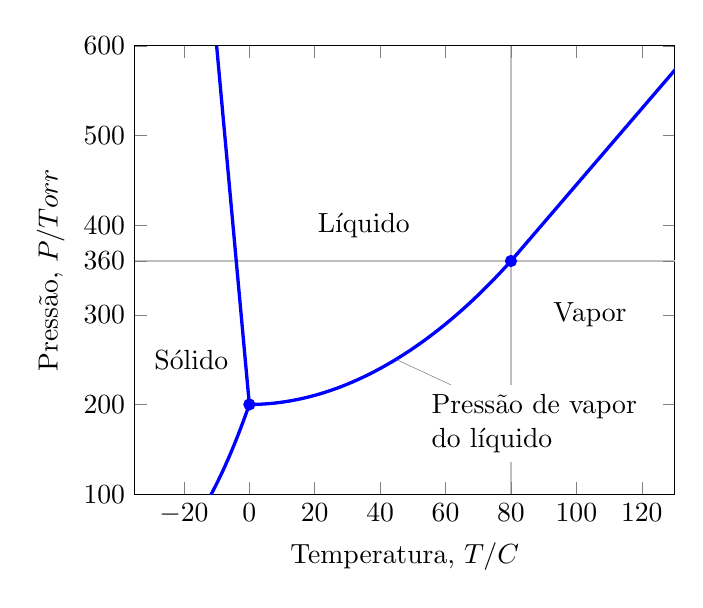
\begin{tikzpicture}
\begin{axis}
        [
            grid = minor,
            ylabel = {Pressão, $P/\unit{Torr}$},
            xlabel = {Temperatura, $T/\unit{\degree C}$},
            ymin=100, ymax=600,
            xmin=-35, xmax=130,
            extra y ticks = { 360 },
            extra y tick style = { grid = major },
            extra x ticks = { 80 },
            extra x tick labels = {},
            extra x tick style = { grid = major },
        ]       
        \draw [draw=blue, very thick]
            (axis cs: -35, 20) parabola 
            (axis cs: 0, 200);
        \draw [draw=blue, very thick]
            (axis cs: 0, 200) --
            (axis cs: -10, 600);
        \draw [draw=blue, very thick]
            (axis cs: 0, 200) parabola 
            (axis cs: 80, 360);
            % (axis cs: 120, 2000);
        \draw [draw=blue, very thick]
            (axis cs: 80, 360) --
            (axis cs: 160, 700);

        \addplot [ mark=*, color=blue, only marks ] coordinates
            { 
                (0, 200)
                (80, 360)
            };

        \node [anchor = west, align = center] at (axis cs:-32, 250) 
            { Sólido };

        \node at (axis cs:35, 400) 
            { Líquido };

        \node [anchor = west] at (axis cs:90, 300) 
            { Vapor };

        \node[coordinate, pin={[fill=white, align=left] below right:{Pressão de vapor \\do líquido}}] 
            at (axis cs:45,250)   {};
\end{axis}
\end{tikzpicture}
    